Farbladung hat drei m\"ogliche Zust\"ande: rot, blau und gr\"un.
Dabei spielt der Zustand der Farbladung f\"ur die St\"arke der starken Wechselwirkung keine Rolle.
Zus\"atzlich zu den drei Zust\"anden der Farbladung gibt es auch drei Zust\"ande der Antifarbladung. 
Die drei Zust\"ande der Antifarbladung sind entsprechend antirot, antiblau und antigr\"un.
Die Kombination der drei (Anti-)Farbladungen, oder die Kombination Farbladung mit passender Antifarbladung ergibt, angelehnt an die Farblehre, die Farbladung wei{\ss}.
Die Farbladung enth\"alt keine Information \"uber die tats\"achliche Farbe der Teilchen.
Teilchen mit dem wei{\ss}en Zustand als Farbladung entsprechen nach au{\ss}en hin farbneutralen Teilchen, auch wenn sie aus farbgeladenen Teilchen aufgebaut sind.
\newline
Quarks, Antiquarks und Gluonen tragen jeweils Farbladung, wodurch sie an der starken Wechselwirkung teilnehmen.
Unter anderem bindet die starke Wechselwirkung Quarks und Antiquarks zu sogenannten Hadronen. %Ungenau formuliert, weil qqbar ist Meson, wir wollen allgemein
Hadronen werden wiederum in sogenannte Baryonen, aufgebaut aus drei Quarks, und sogenannte Mesonen, aufgebaut aus einem Quark-Antiquark-Paar und entsprechende Antiteilchen unterteilt.
In der Natur kommen nur farbneutrale Teilchen vor, es gibt keine freie Farbladung.
Entsprechend gibt es (Anti-)Quarks nur in Zusammenschl\"ussen und nicht frei. 
Dieses Ph\"anomen wird als \textit{Confinement} bezeichnet.
Um das \textit{Confinement} besser verstehen zu k\"onnen wird im Folgenden das Potential der starken Wechselwirkung betrachtet.
\newline
Die Wechselwirkung, die auf ein Quark-Antiquark-Paar wirkt, folgt aus einem Potential $V(r)$, das einen anziehenden Teil und einen abstoßenden Teil besitzt.
Es gilt \cite{HennerSkript}:
%Der anziehende Teil weist dabei eine Proportionalit\"at zum Abstand $r$ zweier farbgeladener Teilchen auf, w\"ahrend der absto{\ss}ende Teil eine Antiproportionalit\"at zu $r$ aufweist.
%Der absto{\ss}ende Teil ist zus\"atzlich proportional zur sogenannten Kopplungskonstante der starken Wechselwirkung $\alpha_\text{s}$.
\begin{align} \label{eq:Potential}
V(r) = -\frac{4}{3}\frac{\alpha_\text{s}}{r} + kr 
\end{align}
Der absot{\ss}ende Teil $-\frac{4}{3}\frac{\alpha_\text{s}}{r}$ verh\"alt sich proportional zur sogenannten Kopplungskonstante der starken Wechselwirkung $\alpha_{\text{s}}$ und antiproportional zum Abstand $r$ zwischen Quark und Antiquark.
Anders als die Bezeichnung vermuten l\"asst ist die Kopplungskonstante der starken Wechselwirkung nicht konstant, sondern proportional abh\"angig von $r$.
Aufgrund dieses Verhaltens der Kopplungskonstante bez\"uglich $r$ nennt man $\alpha_\text{s}$ auch laufende Kopplungskonstante.
\newline
Der anziehende Teil des Potentials $+kr$ hingegen weist ein lineare Abh\"angigkeit von $r$ auf.
Der Vorfaktor $k$ wird als Stringspannung bezeichnet und liegt in der Gr\"o{\ss}enordnung von etwa 1 GeV/fm.
F\"ur gro{\ss}e Abst\"ande dominiert der anziehende Teil, je weiter die beiden Teilchen also voneinander entfernt sind, umso mehr Energie wird ben\"otigt um den Abstand weiter zu vergr\"o{\ss}ern.
Ab einem bestimmten Punkt wird die ben\"otigte Energie so gro{\ss}, dass sie ausreicht um ein weiteres Quark-Antiquark-Paar zu erzeugen.
Es liegen dann zwei Quark-Antiquark-Paare vor.
Deshalb k\"onnen Quarks nicht direkt einzeln gemessen werden.
\newline
F\"ur kleine $r$ und somit auch kleine $\alpha_\text{s}$ hingegen dominiert der absto{\ss}ende Teil.
Bei einer hohen Dichte von Hadronen wird nach aktuellem Wissensstand davon ausgegangen, dass sich die Hadronen \"uberlappen.
In der \"Uberlappregion k\"onnen sich die Quark und Antiquarks frei bewegen.
Den Zustand f\"ur kleine $\alpha_\text{s}$ nennt man asymptotische Freiheit, da sich innerhalb dieses Zustands Quarks und Antiquarks quasi frei bewegen k\"onnen.
Um so einen Zustand erzeugen zu k\"onnen braucht man eine hohe Dichte von Quarks und Antiquarks oder eine hohe Temperatur.
Eine verbreitete theoretische Beschreibung eines Mediums in diesem hei{\ss}en und dichten Zustand ist das sogenannte Quark-Gluon-Plasma, kurz QGP.
\newline
Ein solcher hei{\ss}er und dichter Zustand kann kurz nach der Kollision von zwei hochenergetischen Atomkernen entstehen.
Quarks und Gluonen, die aus diesem Medium kommen, werden w\"ahrend der sogenannten Hadronisierung wieder zu Hadronen.
Diese Hadronen k\"onnen zerfallen, insofern sie keine stabilen Teilchen sind.
Es kann auch zu ganzen Zerfallsketten kommen, bis die Endteilchen nicht mehr zerfallen.
Je nach dem, wie schnell Teilchen zerfallen, k\"onnen entweder diese oder ihre Zerfallsprodukte gemessen werden und geben indirekt Aufschluss auf Eigenschaften des hei{\ss}en und dichten Mediums.
\newline
Bei der Erforschung des hei{\ss}en und dichten Mediums, beziehungsweise der Suche nach dem QGP, spielt das Phasendiagramm stark wechselwirkender Materie eine wichtige Rolle.
\begin{figure}[thp]
\centering
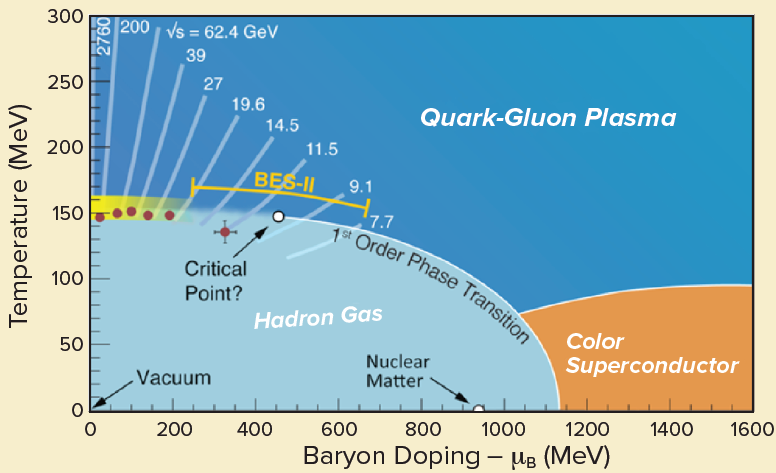
\includegraphics[width=.7\linewidth]{QGPPhaseDiagram.png}
\caption{Phasendiagramm stark wechselwirkender Materie in Abh\"angigkeit der Baryonendichte $\mu_{\text{B}}$ und der Temperatur $T$.
\cite{PAPER:1}}
\label{fig:QGPPhase}
\end{figure}
Abbildung \ref{fig:QGPPhase} skizziert ein Phasendiagramm stark wechselwirkender Materie in Abh\"angigkeit der Baryonendichte $\mu_{\text{B}}$ und der Temperatur $T$.
Bei geringer Baryonendichte und niedriger Temperatur, wie etwa Raumtemperatur, sind alle Quarks und Gluonen in Hadronen gebunden.
Erh\"oht man die Temperatur, oder beide Gr\"o{\ss}en, stark wird ein \"Ubergang in das QGP erwartet, in welchem sich die Quarks und Gluonen quasi frei bewegen k\"onnen.
Au{\ss}erdem muss die Energiedichte gro{\ss} genug sein um ein QGP erzeugen zu k\"onnen, weshalb davon ausgegangen wird, dass sich dieses nur bei Kernkollisionen ausbilden kann.
Proton-Proton-Kollisionen werden als Referenzmessungen benutzt.
\newline
In der Abbildung sind zus\"atzlich verschiedene sogenannte Schwerpunktsenergieen $\sqrt{s}$ eingezeichnet.
Die Schwerpunktsenergie eines Kollisionsexperiments gibt an, wie viel Energie dem System bei der Kollision zur Verf\"ugung steht.
Entsprechend h\"angt $\sqrt{s}$ von der Energie der kollidierende Teilchen oder Kerne ab.
F\"ur Kollisionsexperimente zweier identischer Teilchen oder Kerne mit gleicher Energie $E$ gilt:
\begin{align}
\sqrt{s} = 2E \label{eq:sqrts}
\end{align}
Unterschiedliche $\sqrt{s}$ liefern also Daten aus unterschiedlichen Bereichen des Phasendiagramms.
Um die Bereiche des Phasendiagramms innerhalb des QGP und dem \"Ubergang zwischen quasi freien zu gebundenen Quarks und Gluonen untersuchen zu k\"onnen, werden also Kollisionen mit ausreichenden Schwerpunktsenergieen ben\"otigt.
Der Aufbau eines Kollisionsexperiments wird in Abschnitt \ref{s3} n\"aher erl\"autert.


%F\"ur gro{\ss}e $r$ wird der anziehende Teil also immer stärker.
%Will man also zwei farbgeladene Teilchen wie etwa ein Quark-Antiquark-Paar von einander trennen, so m\"usste man immer mehr Energie aufwenden, je weiter man die Teilchen von einander entfernt.
%Diese Erzeugung eines neue Quark-Antiquark-Paares findet immer statt sobald sie m\"oglich ist.
%Deshalb sind Quarks und Gluonen nicht direkt einzeln messbar, was die Untersuchung von Quarks, Gluonen und der starken Wechselwirkung erschwert.
%Um zu erkl\"aren, wie die starke Wechselwirkung, Quarks und Gluonen trotzdem untersuchen werden k\"onnen muss man sich $\alpha_\text{s}$ genauer anschauen. 
%\begin{figure}[thp]
%\centering
%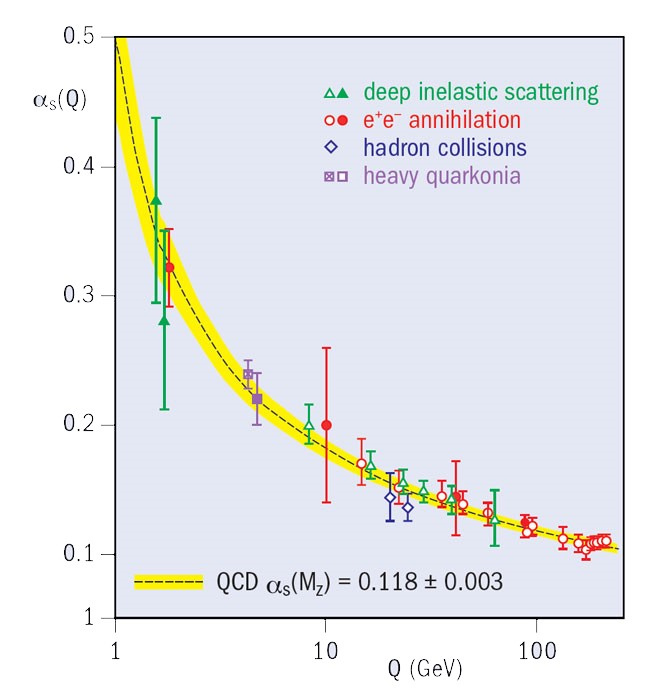
\includegraphics[width=.5\linewidth]{alpha_s.jpg}
%\caption{Die Kopplungskonstante der starken Wechselwirkung $\alpha_\text{s}$ in Abh\"angigkeit des Impulsübertrags $Q$. Eingezeichnet befinden sich Messpunkte unterschiedlicher Experimente, sowie in gelb eine theoretische Rechnung.
%\cite{article:1}}
%\label{fig:alpha_2}
%\end{figure}
%Stattdessen h\"angt $\alpha_\text{s}$ vom sogenannten Impulsübertrag $Q$ zwischen zwei Teilchen ab.
%Abbildung \ref{fig:alpha_2} zeigt den Verlauf von $\alpha_\text{s}$ in Abh\"ahngigkeit von $Q$.
%Der Impulsübertrag $Q$ h\"angt dabei selbst \"uber die De-Broglie-Wellenl\"ange mit dem Abstand $r$ zusammen.
%Es gilt $Q = \frac{h}{\lambda}$, wobei $\lambda$ die r\"aumliche Aufl\"osung beschreibt.
%F\"ur eine genau Aufl\"osung, also f\"ur  sehr kleine $r$ muss entsprechend $Q$ gro{\ss} sein.
%$\alpha_\text{s}$ h\"angt also antiproportional von $r$ ab.